\section{C++ Design, Integration, and Performance}

\subsection{Porting against a behavioral reference}

The native work began with a bounded contract: reproduce the Python book's
state transitions and canonical bytes on the fixed-eight-decimal BTCUSDT
input domain. The June golden vectors were recovered unchanged from commit
\code{578b524}. A library and standalone CLI established operation and
transcript parity before the native book was connected to the Python pipeline.
The integration then addressed the remaining gap between a fast isolated
component and a usable backend for replay, execution, and analysis.

The result is a hybrid implementation. C++ owns price-level storage and book
mutation; Python owns parsing, scheduling, strategy, execution, and research
accounting. This preserves the tested Decimal arithmetic for microprice,
queue fractions, fees, and P\&L while permitting native storage to participate
in the entire application path. It does not imply that the whole simulator has
been translated into C++.

\subsection{Checked fixed-point representation}

Each book side is a \code{std::map<int64_t,int64_t>}. Prices and quantities use
the scale $10^8$; for example, \code{74574.79000000} is stored as
\code{7457479000000}. Direct digit parsing avoids conversion through binary
floating point. Ordered maps provide insertion, replacement, and deletion in
$O(\log N)$ and deterministic best-price and level traversal. RAII containers
own the book memory.

The parser requires unsigned decimal strings with exactly eight fractional
digits, checks scaled-integer overflow, and validates tick/quantity-step
multiples. Stored prices and nonzero quantities must be at least
\code{0.00000100}, where the reference Decimal canonical representation stays
in ordinary fixed-point notation. Signed strings, other Decimal spellings, and
values outside this domain are rejected. Tick and quantity-step metadata can
be normalized exactly by the Python adapter; incoming levels must still obey
the native contract.

Snapshots replace both sides and skip zero quantities. Diffs replace nonzero
quantities and erase zero levels, including absent levels without error.
Duplicate prices retain the reference input-order behavior. Crossed books
remain representable. Both sides of an operation are validated before a
rejected input can mutate state. Allocation failure during an otherwise valid
diff is terminal; the contract does not promise that the same book can be
reused after \code{std::bad_alloc}.

Canonical JSON preserves Python's key order, price order, eight-decimal level
strings, and update ID. OpenSSL EVP computes SHA-256. A transcript digest
hashes the ASCII state hash after every operation, including the initial empty
state. Comparing only the final book could miss divergence that later
reconverges; the transcript cannot conceal an unequal intermediate state.

\subsection{The Python/native boundary}

\code{cpp/src/python_module.cpp} supplies a CPython extension without a second
binding framework. A capsule owns one C++ book and releases it with Python
object lifetime. Exceptions map to Python errors. Calls retain the GIL; the
binding is not a mechanism for parallel execution within one Python process.

\code{src/replay/cpp_orderbook.py} implements \code{CppOrderbook} against the
reference book interface. It keeps no mirrored \code{SortedDict}. After an
update, one native return refreshes cached best bid/ask prices and quantities,
counts, update ID, and sequence. Those public price and quantity values become
Python \code{Decimal} objects. Inherited mid, spread, and microprice formulas
therefore execute with the same arithmetic as the reference. Price-level
quantity and ordered-level accessors query native storage for execution logic
and diagnostics.

The shared backend factory selects Python by default and C++ explicitly.
\code{--book-backend cpp} is propagated through replay, comparison,
reconciliation, microprice and OFI analysis, and panel orchestration. A missing
or invalid native module fails clearly; it does not silently select Python.
The loader checks the extension API and hashes the loaded binary. Backend
identity, instrument-grid metadata, native build identity, and reference
source identity travel with provenance and cache keys. Native outputs use a
separate namespace so a backend experiment cannot overwrite frozen V3
research artifacts.

This division is intentional. Reimplementing proportional queue arithmetic or
P\&L using rounded native fixed-point operations would introduce a new
behavioral problem before proving storage equivalence. The present boundary
keeps derived arithmetic unchanged and measures the conversion overhead it
actually incurs.

\subsection{Layered parity evidence}

Native CTest checks decimal boundaries, overflows, invalid-input rejection,
snapshot/diff behavior, and hashing. Address/undefined-behavior sanitizer
checks exercise the native implementation. Differential tests compare the
unchanged golden operations, seeded random traces containing deletes,
duplicates, resets and crossed states, and every canonical state in a real
development-hour trace.

The isolated recorded-hour test applies 35,999 operations and matches all
\NativeRecordedStates{} states, including the empty book. Its transcript
digest is
\begin{lstlisting}
eec2fd20873bc2105d342ca3b5fe5736941007fcd087eb3eeb6c4140e5fd8731
\end{lstlisting}
The final state hash is
\begin{lstlisting}
8acb43778de91b3029ed91e83280a9c4429146303257f5a7be45ec9d54f12dff
\end{lstlisting}

Pipeline validation goes beyond equal book hashes. The differential runner
compares complete streams of checkpoints, order events, fills, book samples,
markouts, queue diagnostics, population and fill-conditioned OFI samples, plus
hold time, P\&L, statistics, final inventory, fees, and final book. Backend
identity may differ; execution semantics may not. Inputs are accepted only
from the hash-matching frozen development inventory. Holdout data is excluded
from this engineering validation.

The first recorded pipeline comparison exposed why this extra layer matters:
an absent price-level lookup became Decimal \code{0E-8} in the adapter while
the reference returned Decimal \code{0}. Those values are numerically equal,
but their string representations differed in order-event and queue-diagnostic
streams. Returning the reference's canonical zero corrected the discrepancy.
Final book equality or a P\&L-only comparison would not have caught it.

% Generated from verified native pipeline artifacts; do not edit.
Native storage matched Python across all 120 selected development hours and 240 hour/endpoint runs. The comparison hashes every order event, fill, book sample, markout, queue diagnostic, OFI population and conditional sample, and final accounting state. It also checks hold-time and P\&L summaries, replay statistics, and book checkpoints every 1,000 market events. All hourly replay statistics, net P\&L, fees, and final positions also match the frozen V3 reconciliation artifacts. No holdout strategy outcomes were evaluated.

\begin{table}[H]
\centering\small
\begin{tabular}{lrrr}
\toprule
Queue endpoint & Python median (s) & Native median (s) & Ratio \\
\midrule
No credit & 5.638 & 4.826 & 1.168\,$\times$ \\
Proportional credit & 5.672 & 4.771 & 1.189\,$\times$ \\
\bottomrule
\end{tabular}
\caption{Integrated pipeline measurements for 12 April 2026, 09:00 UTC. One warmup and three measured repetitions per backend, with alternating backend order and a warm operating-system page cache. Ratios compare the measured medians and need not indicate an overall speedup.}
\label{tab:native-pipeline-timing}
\end{table}

These timings include raw gzip reads and JSON parsing, object construction, replay, strategy callbacks, execution, checkpoint hashing, book samples, markouts, P\&L, hold-time and queue diagnostics, and OFI sample construction. They exclude imports and initial native discovery, parity serialization, object destruction, output writing, pooled regressions, bootstrap inference, and report generation. Every measured repetition is checked against the Python output streams. This is a separately scoped measurement from the preloaded book-update benchmark.


\subsection{Isolated book-update measurement}

The standalone benchmark first verifies transcript parity and then applies
identical preloaded operations. It times book construction, dispatch, decimal
conversion, and updates. Decompression, JSON/protocol parsing, state hashing,
process startup, book destruction, callbacks, and execution are outside the
timed region. Python book destruction was initially capable of falling inside
the next iteration's timer; commit \code{fc07501} corrected that boundary
before the following measurements were accepted.

\begin{table}[H]
\centering
\caption{Standalone book-update timings on 11 September 2026. Intel Core
i5-12400F; Python 3.11.14; GCC 13.3.0 Release, \code{-O3 -DNDEBUG}; one warmup
and five measured repetitions. Ratios compare medians.}
\begin{tabularx}{\textwidth}{@{}L{0.34\textwidth}YYY@{}}
\toprule
Input & Python median & C++ median & Ratio \\
\midrule
Synthetic, 20,000 updates & 85.445115 ms & 6.892484 ms & $12.39685\times$ \\
Recorded hour, 35,999 updates & 623.006815 ms & 45.326177 ms & $13.74497\times$ \\
\bottomrule
\end{tabularx}
\end{table}

\begin{figure}[H]
\centering
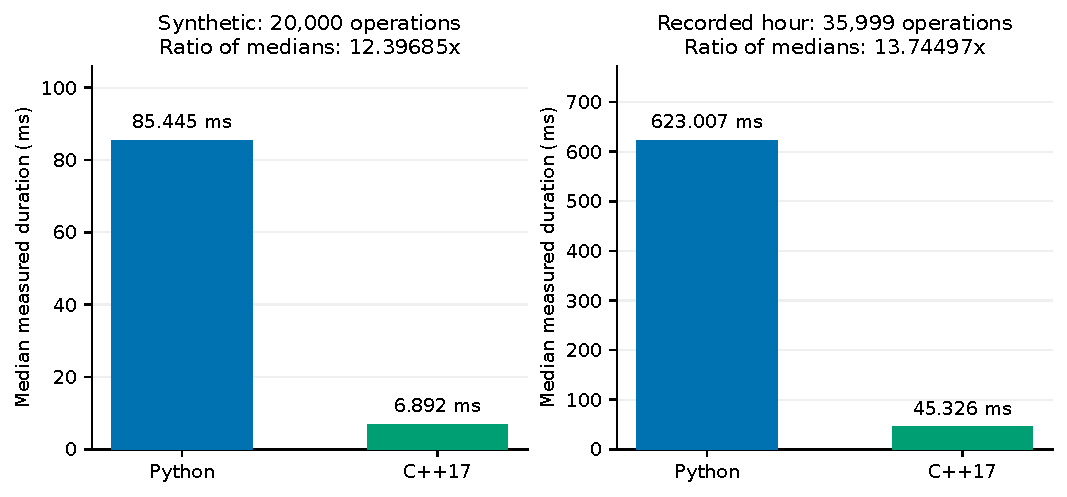
\includegraphics[width=0.92\textwidth]{figures/native_book_benchmark.pdf}
\caption{Parity-gated standalone book-update measurements. These ratios
exclude the CPython adapter and the rest of replay; they must not be reported
as full-application acceleration.}
\label{fig:bookbench}
\end{figure}

The synthetic input has seed 42 and 200 initial levels per side. The recorded
input is the depth hour beginning 12 April 2026 at 09:00 UTC. Python was timed
first and C++ second; all repetitions, environment descriptors, source and
binary hashes, and input identity are retained. These are local performance
measurements, not a general hardware-independent factor.

\subsection{Integrated timing has a different denominator}

\code{scripts/validate_native_pipeline.py} separately times construction,
reopened raw gzip/JSON inputs, replay, strategy, execution, checkpoints, book
sampling, markouts, P\&L, hold-time and queue diagnostics, and OFI sample
construction. Initial imports/module discovery, parity serialization,
destruction, output writing, pooled regression, bootstrap, and report
generation are excluded. Timed repetitions alternate backend order, retain
each duration, and rerun parity against the reference before accepting a
measurement. Reopened inputs are normally served from the warm operating
system page cache.

This broader path includes Python/native conversion and work unaffected by
native storage. Even a large isolated update ratio need not translate to an
application speedup. Reporting a slower or similar integrated result is an
engineering finding about the chosen boundary, rather than a reason to
substitute the isolated microbenchmark for application evidence. The binding
provides a usable native backend; its measured benefit depends on the workload.
